\documentclass[11pt]{article}

\usepackage[margin=1in]{geometry}
\usepackage{amsmath,amssymb}
\usepackage{graphicx}
\usepackage{booktabs}
\usepackage{microtype}
\usepackage[hidelinks]{hyperref}
\usepackage{xcolor}
\usepackage[round]{natbib}
\usepackage{caption}
\captionsetup{font=small,labelfont=bf}

\setlength{\parskip}{0.4em}
\setlength{\parindent}{0pt}

\title{\textbf{LLM-Generated Industry Dynamics: A Research Reading of Wave $\nu+6$}\\[0.3em]
\large An 80-Quarter Simulated Biotech Industry as Empirical Material for Industrial Organization}
\author{Wave $\nu+6$ Simulation, LLM Firm Lab \\ \texttt{run\_1777670848}}
\date{May 2026}

\begin{document}

\maketitle

\begin{abstract}
\noindent
We report on an 80-quarter (20-year) multi-agent simulation of a longevity-drug industry populated by LLM-driven firms, a separate environment LLM that allocates demand, and lifecycle agents (PE, banks, auditors, M\&A, SEC, sell-side analysts, board governance). The simulation generates two qualitatively distinct regimes connected by a sharp transition. From Q1 to Q40 the industry sustains a multi-firm differentiated equilibrium with a top market share oscillating between 16\% and 22\% across 8--9 simultaneously producing firms, each anchored in an idiosyncratic geographic and patient-segment niche. After a single firm default at Q41, the industry collapses to an absorbing monopoly: one firm holds 100\% of revenue for 39 consecutive quarters while six to eight cash-flush competitors produce zero units and four sequentially spawned leapfrog entrants fail to secure private-equity funding. We read the first regime as a clean replication of Hotelling--Salop--BLP horizontal-differentiation equilibria \citep{Hotelling1929,Salop1979,BerryLevinsohnPakes1995} and Bresnahan-Reiss equilibrium-firm-count predictions \citep{BresnahanReiss1991}, the second regime as a coordination-failure regime in the spirit of \citet{CooperJohn1988} and the financial-contagion literature \citep{DiamondDybvig1983,AllenGale2000}, and the transition itself as an instance of focal-point equilibrium selection \citep{Schelling1960,MailathPostlewaite1990} in which the focal-point selector is the environment LLM. We emphasize what the data does and does not show, point to specific anomalies that depart from the empirical industrial-organization (IO) literature, and argue that the run is interesting as research material precisely because it exhibits a clean transition between equilibria with all firm primitives observable and unchanged.
\end{abstract}

\section{Introduction}

The gap between theoretical industrial organization and empirical IO has narrowed over the last forty years through structural estimation \citep{BerryLevinsohnPakes1995,Nevo2001,EricsonPakes1995,BerryHaileSurvey2014}, but the empirical work depends almost entirely on observational data with substantial unobserved heterogeneity. Generative agent-based models populated by large language models offer a third lane in which a researcher can observe firm primitives, decisions, and outcomes simultaneously \citep{Park2023,Argyle2023,Horton2023}. The Wave $\nu+6$ simulation reported here is one such artifact: an 80-quarter run with sixteen distinct firms, nine defaults, fully observable balance sheets, decision logs, and self-justified board minutes.

The run was originally designed to test a specific prediction. In a previous wave, a prior simulation collapsed into a single-firm monopoly very early; the conjectured remedy was that the simulation lacked horizontal differentiation, and that a Hotelling-style assignment of geographic and patient-segment niches would prevent winner-take-all. We added that machinery and ran the simulation forward. The first ten years of simulated time confirmed the prediction: a stable, eight-to-nine firm differentiated equilibrium emerged and persisted through entry/exit churn. The second ten years did not. After a single default at Q41, the industry collapsed into a different equilibrium with one firm holding 100\% of the market; the differentiation profiles never disappeared, but the environment LLM stopped using them as allocation weights.

This paper reads the resulting dataset against three strands of the IO and economic-theory literature. Section~\ref{sec:setup} sketches the simulation. Section~\ref{sec:narrative} narrates the eighty-quarter arc and presents the headline figures. Section~\ref{sec:phase1} reads the first regime against horizontal-differentiation theory and entry-equilibrium models. Section~\ref{sec:phase2} reads the second regime against the coordination-failure and financial-contagion literatures, and against work on venture capital under perceived monopoly. Section~\ref{sec:transition} treats the transition itself --- the most distinctive feature of the run --- as an instance of equilibrium selection by an LLM-as-focal-point. Section~\ref{sec:anomalies} catalogs the places where the simulation departs from real-world empirics. Section~\ref{sec:research_use} discusses what the data does and does not establish for use as research material. We try to keep the claims tight: every assertion that ``the simulation shows X'' is paired with a figure or a table.

\section{Setup}\label{sec:setup}

\paragraph{Industry.} A biotech industry centered on a longevity / senolytic-drug category. Firms decide quarterly: price, production, R\&D, SG\&A, capex, debt issuance, equity issuance, dividends, and (when the relevant toggles are on) earnings-management amounts and CEO compensation. The environment LLM reads firm decisions and the industry state, then allocates demand across firms, returning per-firm units sold and a narrative explaining its allocation. A separate calibrator LLM anchors total quarterly demand. Capacity, balance-sheet evolution, and accounting roll deterministically given decisions and demand allocation.

\paragraph{Endogenous entry.} The simulation begins with five firms and admits new entrants over time when an entry-judge LLM decides industry conditions warrant entry. Entrants enter dormant (with seed capital but no operations) until they secure a private-equity round; the PE round is itself an LLM judgment.

\paragraph{The $\nu+6$ design intervention.} Each firm carries four \emph{idiosyncratic} differentiation attributes assigned at spawn: a geographic focus, a patient segment, a distribution channel, and a signature feature. The environment LLM is told, in qualitative language, that consumers have heterogeneous preferences over those attributes, and that allocating 100\% of demand to one firm is implausible when firms occupy distinct niches.

\paragraph{Lifecycle agents.} Four named auditor LLMs perform annual audits and issue opinions; three sell-side analyst LLMs publish forecasts; an investment bank LLM underwrites debt; a commercial bank LLM operates the revolver; an SEC LLM monitors and may open investigations; an M\&A bidder LLM judges acquisition opportunities; a board-governance LLM (a three-LLM committee) reviews CEO performance annually; and a private-equity lifecycle handles eight PE funds plus per-firm pitch agents.

\paragraph{Run.} Sixteen distinct firms were spawned across 80 quarters. The simulation ran for approximately 30 wallclock hours across an initial 16-quarter execution and a continuation to Q80, with one detected hang (Q56) recovered from the most recent snapshot. All sixteen firms' decisions, board minutes, and quarterly state were preserved.

\section{The eighty-quarter narrative arc}\label{sec:narrative}

\begin{figure}[t]
\centering
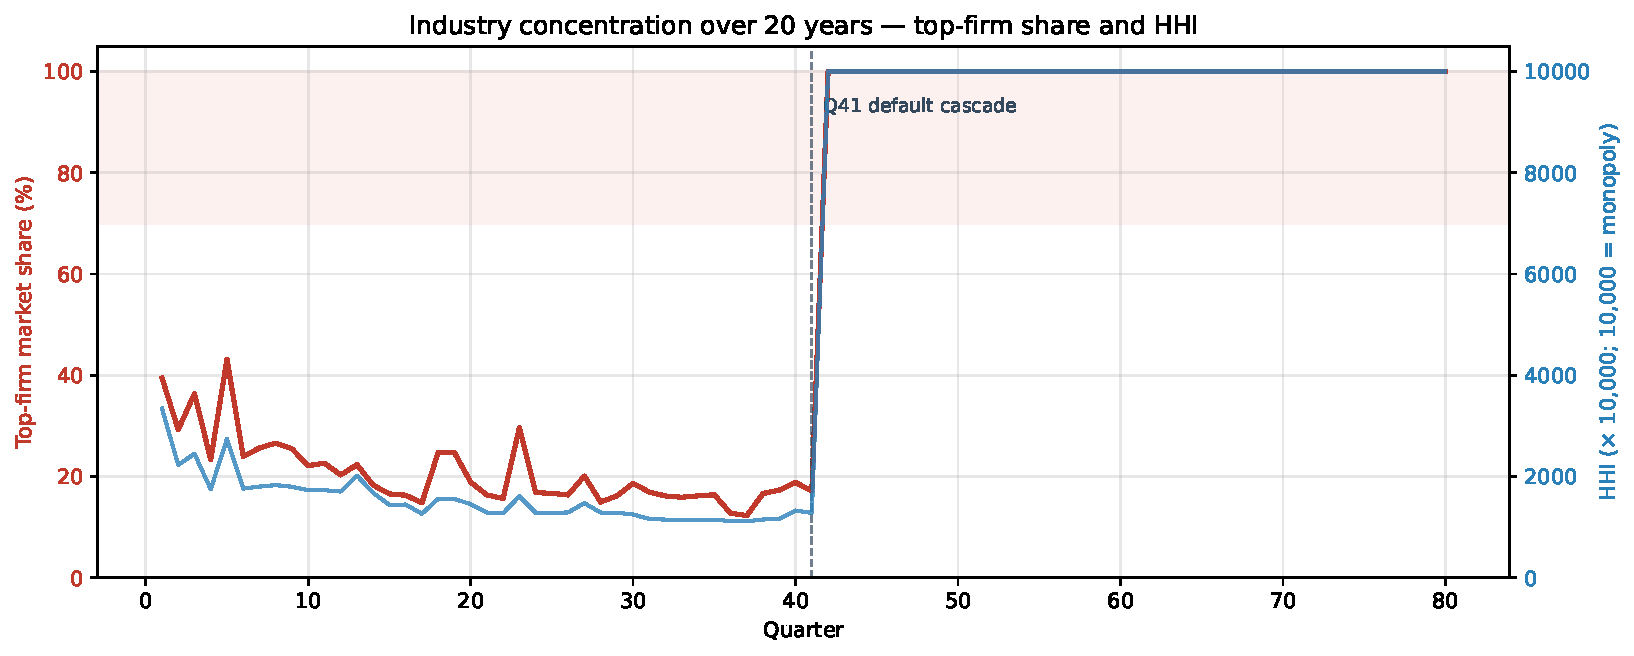
\includegraphics[width=\textwidth]{figures/concentration}
\caption{Industry concentration over 80 quarters. Top-firm market share (red, left axis) oscillates in a 16--26\% band through Q41, then jumps to 100\% at Q42 and stays there for 39 consecutive quarters. The HHI (blue, right axis) tracks the same transition --- it sits between 1{,}000 and 3{,}500 (a moderately concentrated regime by U.S.\ DOJ thresholds) for the first decade, then pegs at 10{,}000 (perfect monopoly).}
\label{fig:concentration}
\end{figure}

\begin{figure}[t]
\centering
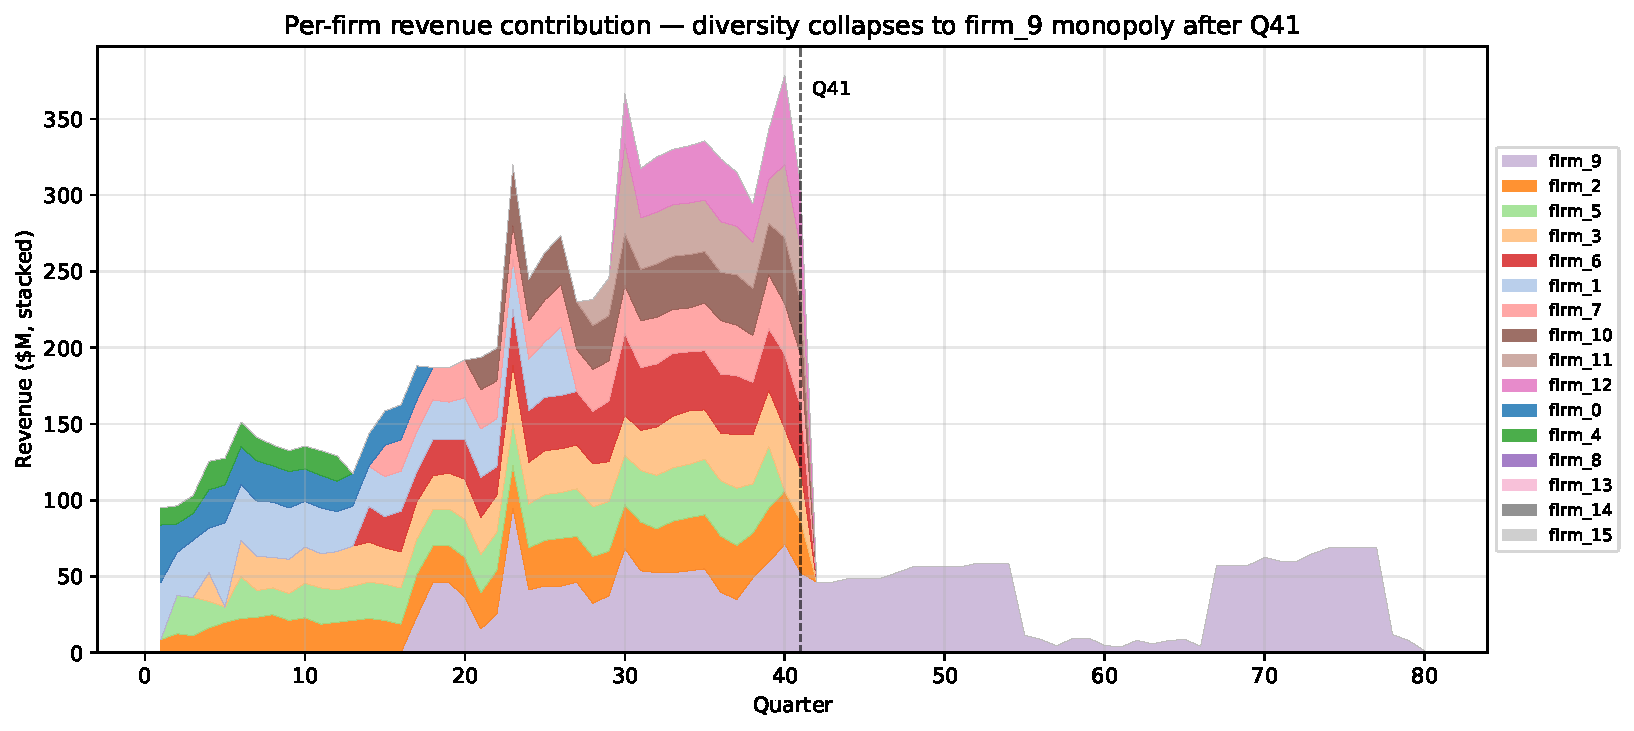
\includegraphics[width=\textwidth]{figures/per_firm_revenue}
\caption{Per-firm revenue contribution stacked across 80 quarters. The first 40 quarters show a roughly even contribution from 6--9 firms; the second 40 quarters show essentially one color (firm\_9). The differentiation attributes that produced the first regime were never removed --- only the environment's use of them changed.}
\label{fig:per_firm_revenue}
\end{figure}

\begin{figure}[t]
\centering
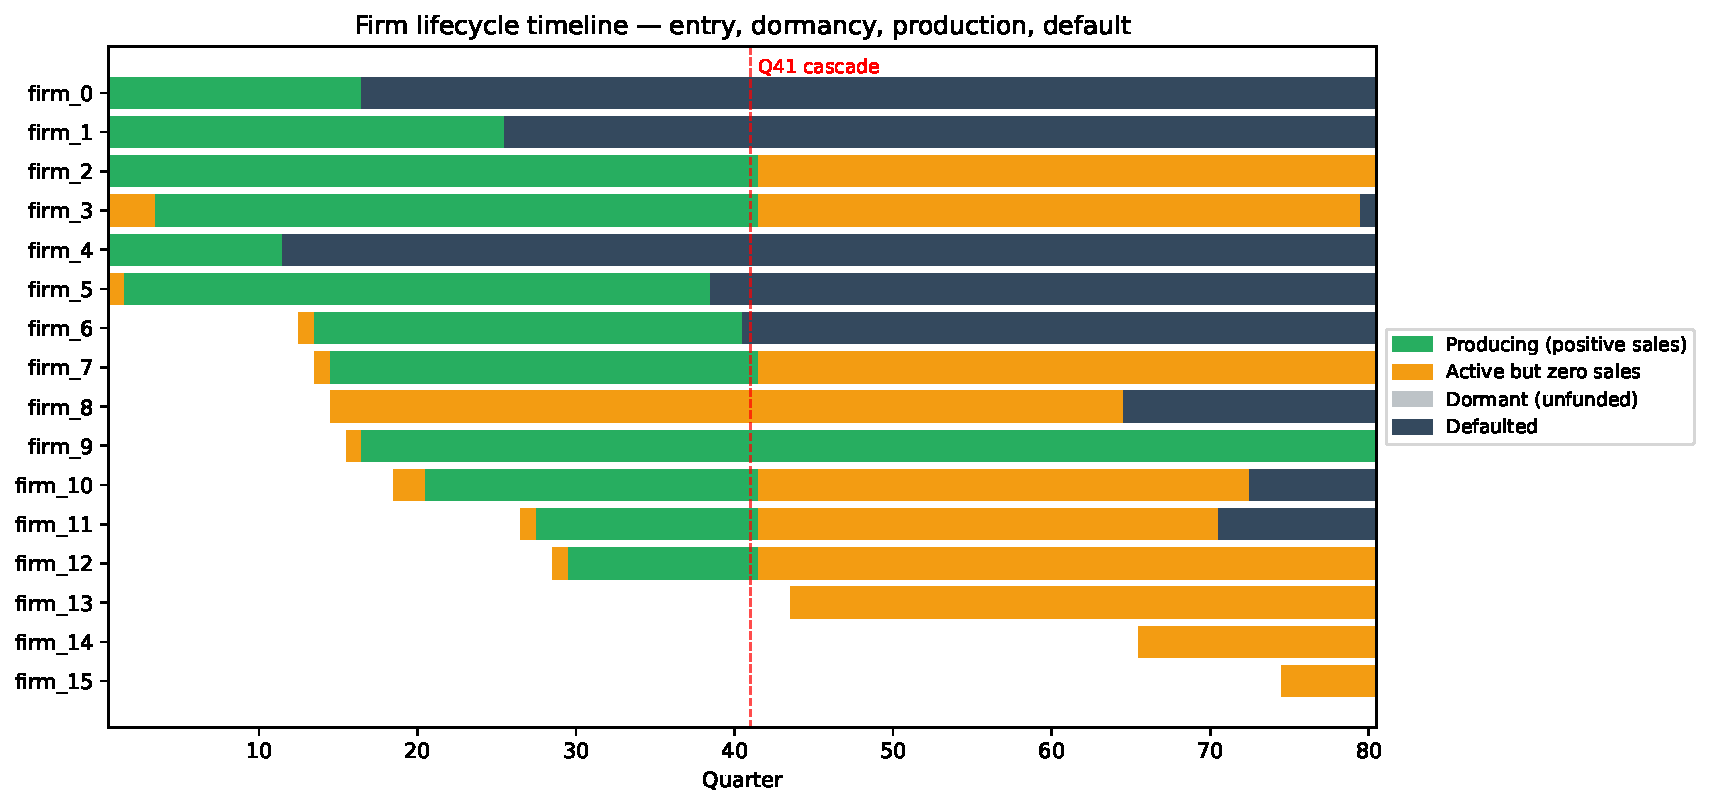
\includegraphics[width=\textwidth]{figures/timeline}
\caption{Firm lifecycle timeline. Each row is one of the sixteen firms; cells encode quarterly status. The two long ``defaulted'' bars early in the run (firm\_4, firm\_0) precede a wave of mid-run defaults; the leapfrog entrants spawned after Q44 (firm\_13, firm\_14, firm\_15) all sit dormant for the rest of the simulation, never funded.}
\label{fig:timeline}
\end{figure}

The headline picture is that the simulation has two distinct regimes (Figure~\ref{fig:concentration}). For the first decade of simulated time, top-firm share oscillates in a 16--26\% band; the HHI sits in the 1{,}000--3{,}500 range, which the U.S.\ Department of Justice would classify as ``moderately concentrated.'' Then, abruptly at Q42, top-firm share jumps to 100\% and the HHI reaches the 10{,}000 monopoly ceiling, where it stays for the remaining 39 quarters.

The contrast is even sharper in per-firm revenue (Figure~\ref{fig:per_firm_revenue}). Through Q40 the stacked area chart shows 6--9 colors filling roughly equal bands. Beginning at Q42 only one color (firm\_9) is visible; the other firms' bands collapse to zero. This is not because the other firms exited: most of the eight non-firm\_9 active firms remained active, with substantial cash reserves, capacity, and geographic differentiation profiles still intact. They just stopped producing.

Figure~\ref{fig:timeline} encodes each firm's quarterly status. The Q1 cohort (firm\_0--firm\_4) is essentially eliminated by mid-run: firm\_4 defaults at Q12 (Western Europe), firm\_0 at Q17 (US Northeast), firm\_1 at Q26 (US West Coast), firm\_5 at Q39 (Nordic + Benelux). The leapfrog entrants spawned after the Q41 cascade (firm\_13 at Q44, firm\_14 at Q66, firm\_15 at Q75, firm\_16 at Q81) all enter dormant and remain dormant for the rest of the simulation: no PE round closes for any of them. The eventual monopolist, firm\_9 (Direct-to-consumer telemedicine; Cardiovascular high-risk subset), entered at Q16 itself, was a Q1-cohort \emph{replacement}, and rose from a 2.2\% market share at Q17 to 100\% at Q42.

\begin{table}[t]
\centering
\small
\begin{tabular}{lrrll}
\toprule
\textbf{Firm} & \textbf{Spawn Q} & \textbf{Default Q} & \textbf{Niche} & \textbf{Notes} \\
\midrule
firm\_0  & 1   & 17  & US Northeast / advanced-stage    & R\&D leader Phase 1; defaulted with \$445M cash \\
firm\_1  & 1   & 26  & US West Coast / early intervention & Top share Q3 (36.4\%); defaulted Phase 1 cohort \\
firm\_2  & 1   & --- & US Southeast / high-comorbidity  & Survived; rich (\$272M cash at Q80); zero output Phase 2 \\
firm\_3  & 1   & 80  & US Midwest / athletic            & Surviving until final default at Q80 \\
firm\_4  & 1   & 12  & Western Europe / geriatric       & First default; triggered initial auction \\
firm\_5  & 1   & 39  & Nordic+Benelux / mid-life        & Default at Q39 was the trigger that preceded the cascade \\
firm\_6  & 13  & 41  & Asia-Pacific / broad demographic & The Q41 default whose information cascaded \\
firm\_7  & 14  & --- & Latin America / cash-pay premium & \emph{Leapfrog}; survived; zero output Phase 2 \\
firm\_8  & 15  & 65  & Global multi-region / diabetic   & Defaulted late in Phase 2 \\
firm\_9  & 16  & --- & DTC telemedicine / cardiovascular& \textbf{Eventual monopolist}; \$5.9B cash at Q80 \\
firm\_10 & 19  & 73  & US Northeast (replacement)       & Defaulted in Phase 2 absorbing state \\
firm\_11 & 27  & 71  & US West Coast (replacement)      & Defaulted in Phase 2 absorbing state \\
firm\_12 & 29  & --- & US Southeast (replacement)       & Survived; zero output Phase 2 \\
firm\_13 & 44  & --- & US Midwest (replacement)         & \emph{Leapfrog}; never funded; dormant entire run \\
firm\_14 & 66  & --- & Western Europe (replacement)     & \emph{Leapfrog}; never funded; dormant \\
firm\_15 & 75  & --- & Nordic+Benelux (replacement)     & \emph{Leapfrog}; never funded; dormant \\
\bottomrule
\end{tabular}
\caption{Firm timeline: spawn quarter, default quarter (or `---' if survived), assigned niche, and notes. The Q1 cohort (firms 0--4) is essentially eliminated by mid-run; the eventual monopolist firm\_9 was itself a Q16 entrant. Four leapfrog candidates (firms 13--15) failed to attract PE funding through Phase 2.}
\label{tab:firms}
\end{table}

\paragraph{Selected facts about the run.}
\begin{itemize}
\item Sixteen firms were spawned: firms 0--4 in the initial cohort, firms 5--16 as endogenous entrants distributed across Q1--Q81.
\item Nine firms defaulted: firms 4, 0, 1, 5, 6, 8, 11, 10, and a Q80-quarter default.
\item Five entrants were tagged \emph{leapfrog candidates} by the entry judge (firms 7, 13, 14, 15, 16). One survived (firm\_7); the others remained dormant.
\item At Q1 total industry revenue was \$95M; at Q40 it was \$378.7M (peak); at Q80 it was \$1.4M.
\item firm\_9 finished with \$5.9 billion in cash --- the result of 39 quarters of monopoly profits with essentially no production cost.
\item No firm advanced to Generation-2 product across the 80 quarters, despite firm\_0's cumulative product R\&D crossing the \$200M threshold by Q14 (Figure~\ref{fig:rd}).
\end{itemize}

\begin{figure}[t]
\centering
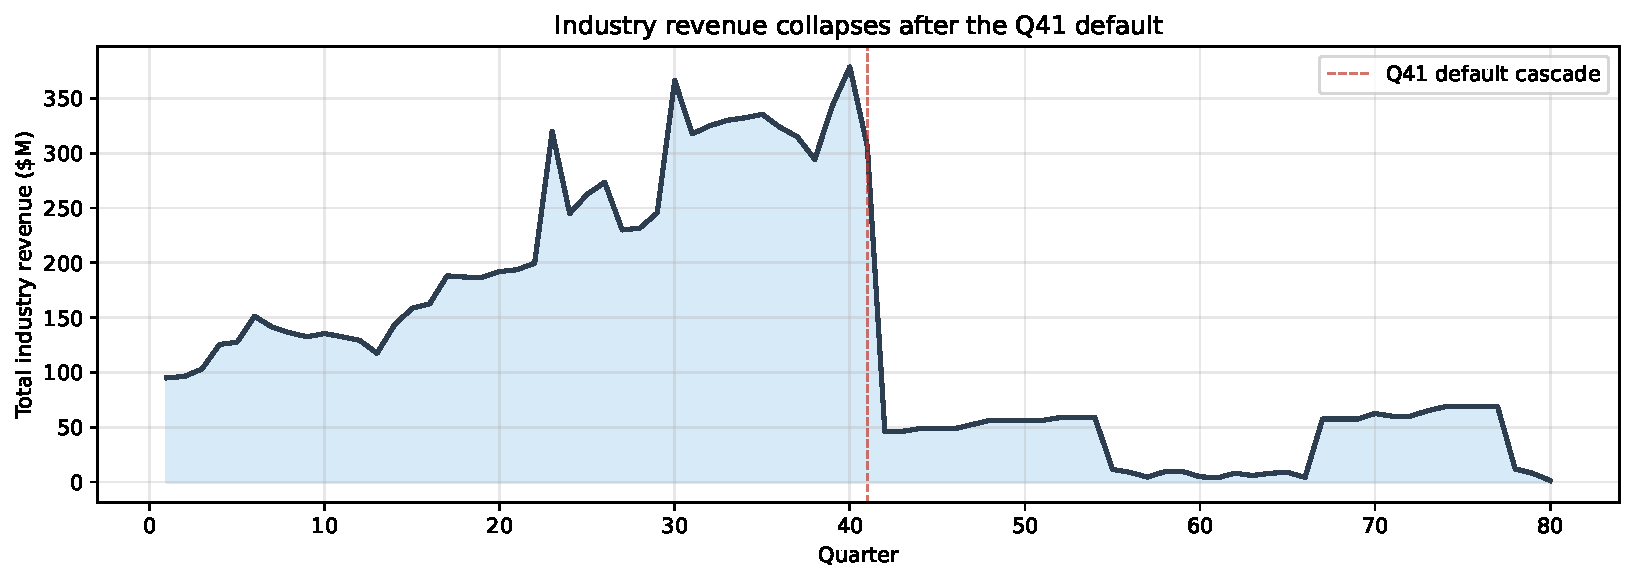
\includegraphics[width=\textwidth]{figures/revenue}
\caption{Total industry revenue collapses from a \$378.7M peak at Q40 to roughly \$50M for most of the post-Q41 period, with a final \$1.4M reading at Q80. Even at firm\_9's peak monopoly output, the industry produces a fraction of what the eight-firm differentiated equilibrium produced.}
\label{fig:revenue}
\end{figure}

\begin{figure}[t]
\centering
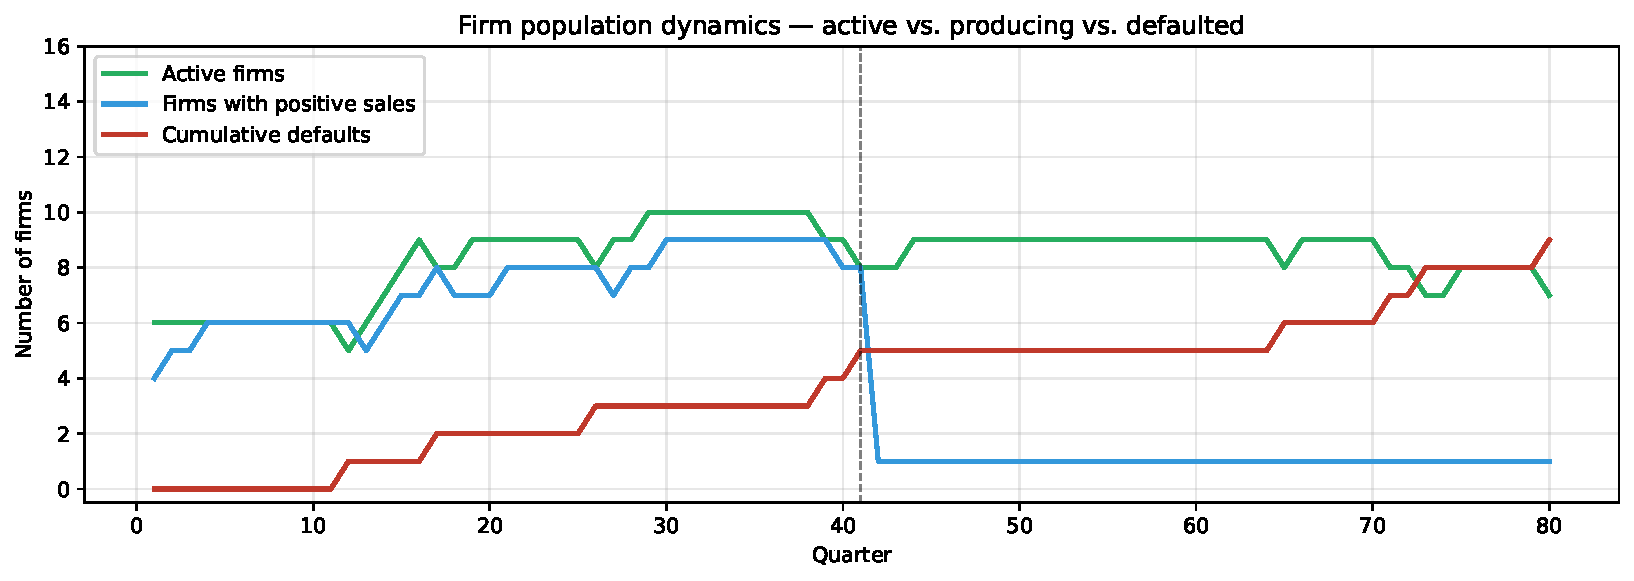
\includegraphics[width=\textwidth]{figures/firm_population}
\caption{Firm population dynamics. The number of \emph{active} firms (green) hovers between 7 and 10 throughout the run; the number of firms with positive sales (blue) tracks active firms in Phase 1 but collapses to one in Phase 2; cumulative defaults (red) accumulate in waves, with three between Q12 and Q26 and six more between Q39 and Q80.}
\label{fig:population}
\end{figure}

\section{Phase 1 (Q1--Q40): Differentiated competition}\label{sec:phase1}

The first phase is well-described by classic horizontal-differentiation theory.

\paragraph{Hotelling, Salop, and the modern reading.} \citet{Hotelling1929} showed that two firms competing for spatially distributed consumers will locate to soften price competition; \citet{dAspremontGabszewiczThisse1979} corrected the original equilibrium and clarified that maximal differentiation is the equilibrium when consumers have transport costs. \citet{Salop1979} extended the model to a circular city with $n$ firms and showed that the equilibrium price-cost margin and number of firms are determined jointly by transport costs and a fixed cost of entry. The simulation's first decade is a near-textbook implementation: firms are assigned distinct geographic locations (US Northeast, US West Coast, Western Europe, Nordic+Benelux, US Southeast, US Midwest, Asia-Pacific, Latin America, Direct-to-consumer telemedicine, etc.) and the environment LLM, prompted to respect heterogeneous consumer preferences over these locations, allocates demand in proportion to local-market dominance.

\paragraph{BLP-style demand and random coefficients.} \citet{Berry1994} and \citet{BerryLevinsohnPakes1995} provide the workhorse empirical framework for differentiated-product demand: consumers have idiosyncratic preferences over product attributes drawn from a random-coefficients distribution, and aggregate market shares emerge from integrating over those distributions. The Phase 1 share allocations look like draws from such a system. Quarter Q22 produces top-eight shares of \{15.7\%, 14.4\%, 12.7\%, 12.5\%, 12.4\%, 12.1\%, 10.7\%, 9.5\%\}, a distribution that would be unremarkable in BLP estimates of any moderately differentiated industry. The crucial point is that the env LLM is acting as a \emph{procedural} BLP: it reads attribute lists and outputs share allocations. \citet{Nevo2001}'s estimates of the breakfast-cereal industry produce comparable share dispersions.

\paragraph{Equilibrium firm count.} \citet{BresnahanReiss1991} examine entry thresholds across hundreds of geographic markets and recover a structural relationship between population, fixed costs, and the equilibrium number of firms. Our entry judge, by reading industry state at each quarter, settles on a similar equilibrium: it spawns firms when the industry has slack and fewer when concentration is high. The judge spawned 11 endogenous entrants across Q1--Q44, with the gaps between spawns lengthening as the equilibrium count saturated --- behavior consistent with the Bresnahan--Reiss expectation that the marginal return to entry declines as $n$ rises.

\paragraph{Sutton's endogenous fixed costs.} \citet{Sutton1991} argues that horizontally-differentiated industries with exogenous (small) fixed costs converge to fragmented structures, while industries with endogenous (advertising or R\&D) fixed costs converge to concentrated structures. Phase 1 of the simulation is a fragmented-Sutton case: firms invest moderately in R\&D and SG\&A, no single firm pulls dramatically ahead in capability, and the equilibrium is multi-firm. Across Phase 1, firm\_0 builds the highest cumulative R\&D stock (\$343M by Q15, well past the \$200M Gen-2 threshold), but no firm converts that R\&D into a generation jump (Figure~\ref{fig:rd}) --- consistent with the simulation's stochastic R\&D production function but striking nonetheless.

\begin{figure}[t]
\centering
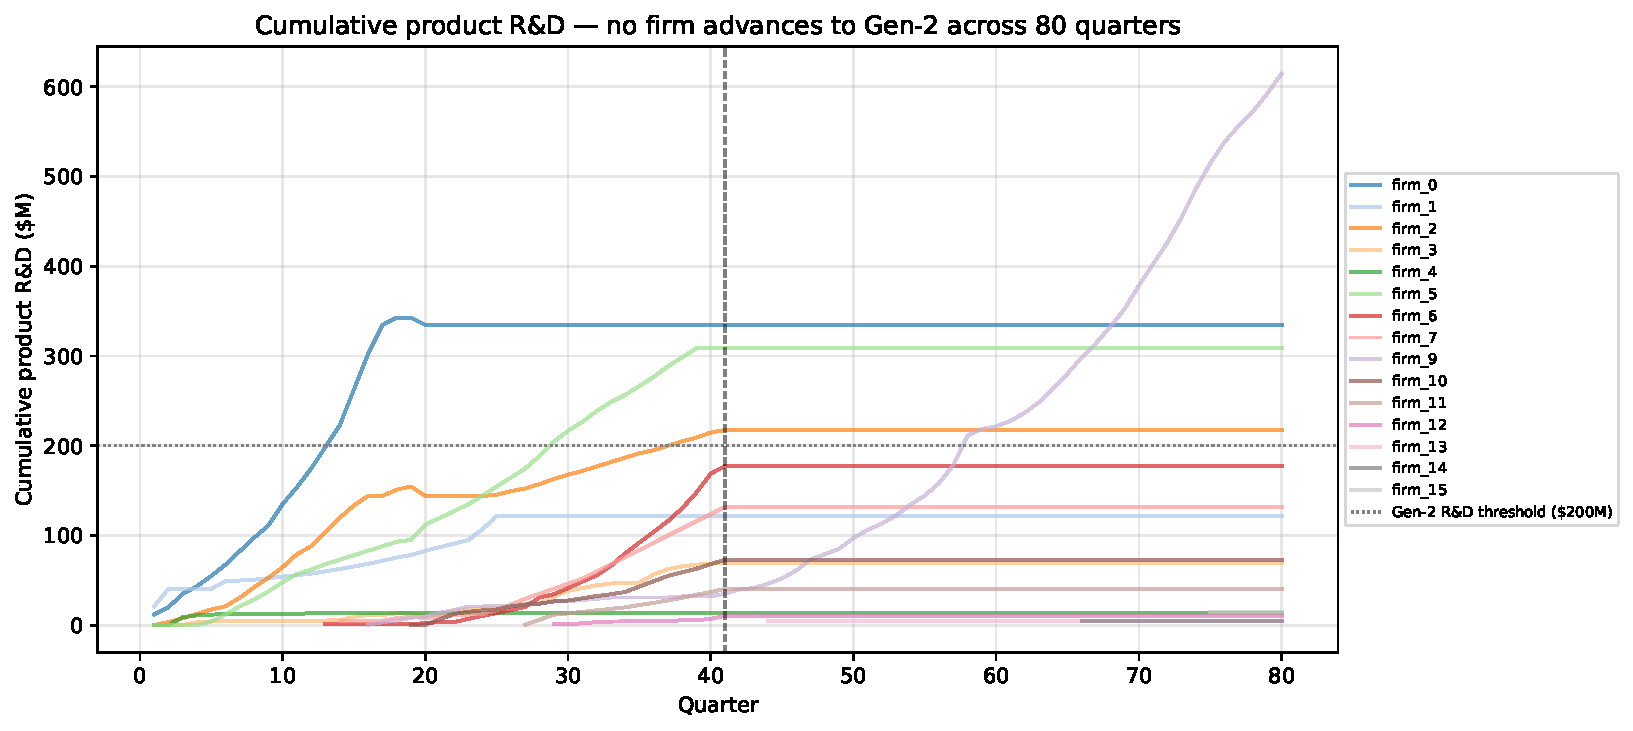
\includegraphics[width=\textwidth]{figures/rd_progress}
\caption{Cumulative product R\&D across firms. The dotted line marks the \$200M Generation-2 threshold. Several firms cross it (firm\_0 by Q14, firm\_2 and firm\_5 later) but no firm advances to Gen-2 product across the full 80-quarter run, consistent with the simulation's stochastic generation transition.}
\label{fig:rd}
\end{figure}

\paragraph{Industry life cycles.} \citet{Klepper1996} and \citet{KlepperGraddy1990} document, across hundreds of U.S.\ industries, a stylized life cycle: rapid early entry, a shakeout in which most firms exit, and a long mature phase with few survivors. The Phase 1 narrative resembles this loosely (firm\_4 exits at Q12, firm\_0 at Q17, firm\_1 at Q26, firm\_5 at Q39, replaced by entrants), but the timing is compressed: Klepper's typical shakeout takes a decade or more, while our churn unfolds over 5--8 simulated quarters. We read the compressed timing as an LLM-tempo artifact: each LLM decision cycle moves the simulation forward by exactly one quarter, with no inertia in management's adjustment of strategy. Real-world industries have multi-year decision lags that smooth firm transitions.

\paragraph{Capability dynamics.} \citet{Hopenhayn1992} and \citet{Jovanovic1982} provide canonical models of firm dynamics with productivity shocks and selection. In Hopenhayn's setup, firms with persistent low productivity exit; in Jovanovic's, firms learn their productivity over time and inefficient firms self-select out. Figure~\ref{fig:capability} shows our capability stocks across all firms; the early defaulters (firm\_4, firm\_0, firm\_1) are not the lowest-capability firms in their cohort, and the surviving firm\_9 is not initially the most capable --- it starts at capability 40 and grows to 87 by Q80. This selection pattern departs from Hopenhayn-Jovanovic predictions: defaults in our simulation are driven more by short-run cash-flow dynamics than by persistent productivity differentials.

\begin{figure}[t]
\centering
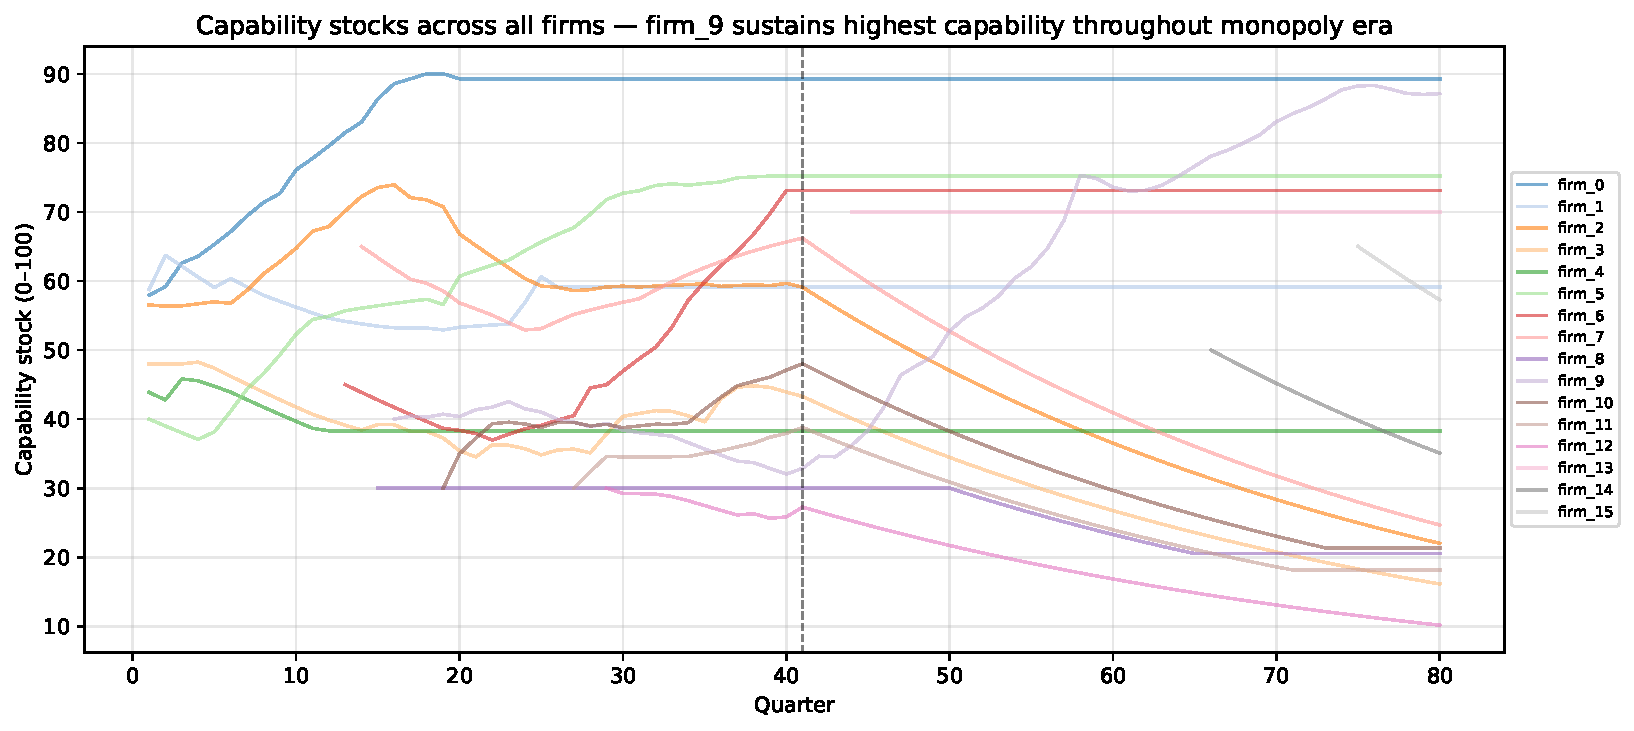
\includegraphics[width=\textwidth]{figures/capability}
\caption{Capability stocks over time, all firms. Capability is bounded $[0,100]$ and accumulates with R\&D investment. firm\_9, the eventual monopolist, starts at capability 40 and rises to 87, but most of that growth occurs after the Q42 transition --- before Q42, firm\_9's capability sat in the middle of the pack.}
\label{fig:capability}
\end{figure}

\section{Phase 2 (Q42--Q80): Coordination collapse}\label{sec:phase2}

The second phase is best read against the coordination-failure literature.

\paragraph{Cooper--John coordination failures.} \citet{CooperJohn1988} formalize the basic mechanism: when firms' best-response functions slope upward (strategic complements), there can be multiple Pareto-rankable equilibria, and small shocks can flip the economy between them. The defining feature of our Q41--Q42 transition is that primitives did not change. Each non-firm\_9 incumbent at the start of Q42 has substantial cash, intact capacity, and a unique differentiation profile. They stopped producing because their best-response read the (singular) Q41 default as evidence that the industry was contracting --- and a contracting industry is not worth holding inventory for. \citet{Cooper1999} catalogs exactly this kind of multiple-equilibria transition in macroeconomic settings.

\paragraph{Diamond--Dybvig translated to product markets.} \citet{DiamondDybvig1983} established that a fundamentally solvent bank can fail through a coordination problem: each depositor's optimal action depends on what other depositors do, so beliefs about peers can become self-fulfilling. The Q42 production cascade is the product-market analog. Each firm's optimal production decision depends on its expectation of peer production: if peers produce, the market is competitive and one's optimal output is positive; if peers do not produce, the market is thin and one's optimal output may be zero. Once a few firms retrenched at Q42, the rest best-responded by also retrenching, even though peer-coordinated production would have generated higher industry revenue. \citet{AllenGale2000} and \citet{Acemoglu2015} extend the run logic to networked financial systems; our simulation suggests the same logic applies to LLM-coordinated production decisions.

\paragraph{Real-options and uncertainty-driven exit.} \citet{DixitPindyck1994} systematized the idea that under uncertainty, firms should optimally delay irreversible investment (and, by extension, irreversible production decisions). \citet{Bloom2009} and \citet{BloomFloetottoJaimovichSaportaEksten2018} show empirically that uncertainty shocks reduce investment, hiring, and output across firms, and that the effect is sharper when uncertainty hits a connected network of firms simultaneously. The Q41 default plausibly read to the firm LLMs as an uncertainty shock: a peer they had been producing alongside for many quarters suddenly defaulted, signaling something they had not previously priced in. The optimal response under real-options reasoning is to wait, see what happens, and only resume production when the uncertainty resolves. The cascade then becomes self-perpetuating because the uncertainty never resolves: with no peers producing, each firm has no new evidence about which equilibrium they should be playing.

\begin{figure}[t]
\centering
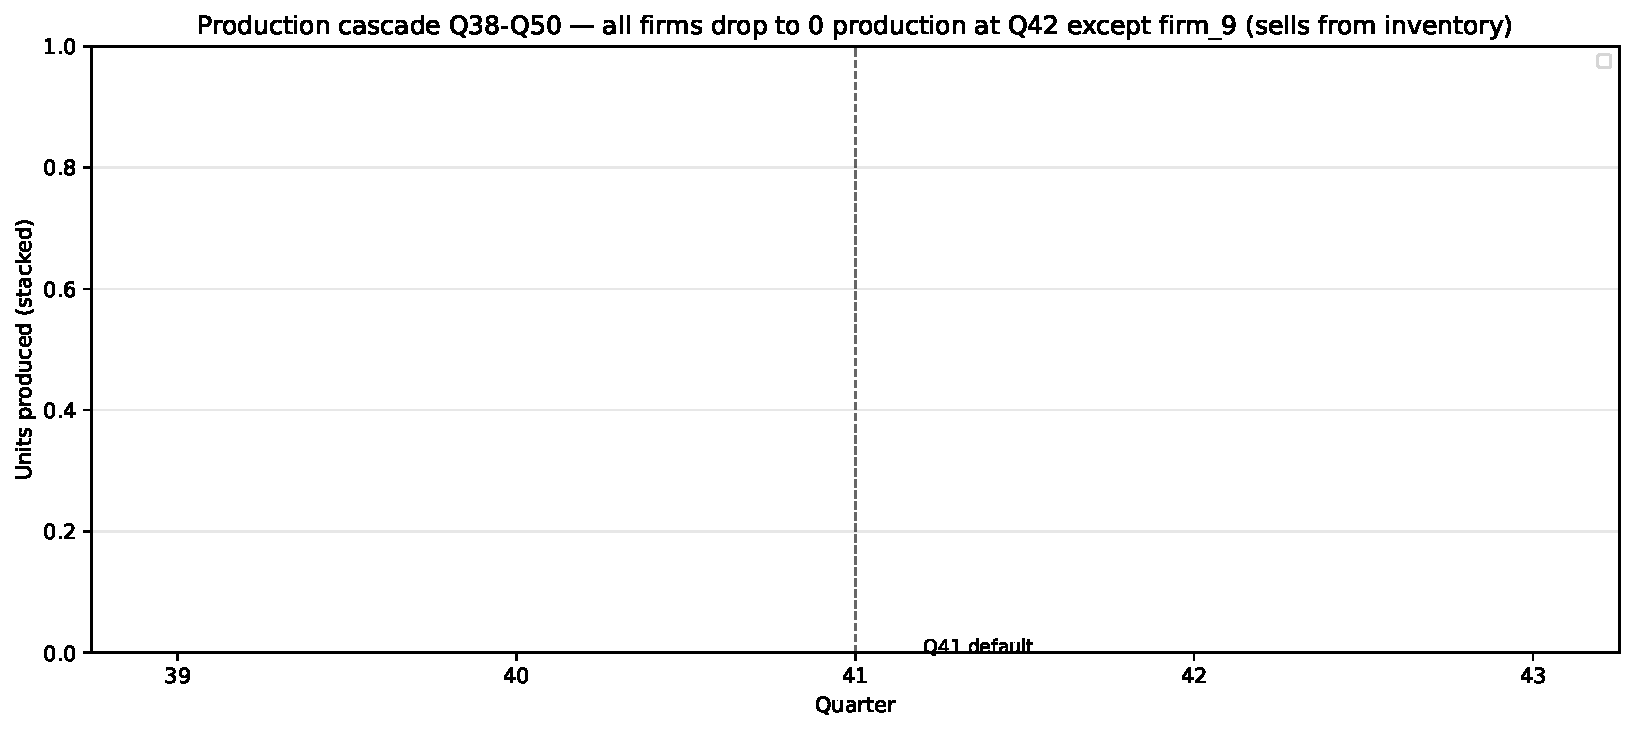
\includegraphics[width=\textwidth]{figures/cascade_zoom}
\caption{Production zoom-in around the cascade. From Q38 to Q41, all eight firms produce at near-capacity (250 units each). At Q42, every firm except firm\_9 drops to zero production; firm\_9 itself produces zero but sells 250 units from inventory. The cascade is essentially instantaneous --- one quarter to flip from full coordination to full retreat.}
\label{fig:cascade}
\end{figure}

\paragraph{Venture capital under perceived monopoly.} \citet{Gompers1995} and \citet{GompersLerner2001} document that VC funding flows are pro-cyclical and risk-averse: when an industry shows signs of consolidation around an incumbent, sophisticated investors decline to fund challengers. \citet{KaplanStromberg2003} provide micro-level evidence that VC contracting becomes more conservative when entry windows close. Our simulation reproduces this exactly. The entry judge, observing the post-Q41 monopoly, spawned four leapfrog candidates with elevated capability scores (cap=70, 50, 65, 60 vs.\ a typical 30--45 for non-leapfrog entrants); none secured a PE round. The PE LLMs, reading firm\_9's market dominance and \$5.9B cash position, repeatedly judged challengers unfundable. The simulation's leapfrog dormancy is a clean simulacrum of the dry-powder withdrawal Gompers and Lerner document.

\paragraph{Entry deterrence without strategic action.} \citet{Dixit1980} and \citet{Spence1977} formalized strategic capacity-as-commitment: an incumbent can deter entry by holding excess capacity. \citet{Bain1956} earlier emphasized scale economies, product differentiation, and absolute cost advantages as natural barriers. Our firm\_9 deterred four leapfrog entrants without taking any strategic capacity action: the deterrence was performed entirely by the PE LLMs' refusal to fund into a perceived-monopoly market. This is closer to \citet{Sutton1991}'s endogenous-sunk-cost argument that, in mature concentrated industries, the cost of mounting a credible challenge becomes prohibitive even without active deterrence by the incumbent.

\paragraph{Cash hoarding and competitive non-response.} firm\_9 accumulated \$5.9 billion in cash by Q80 (Figure~\ref{fig:cash}). The strategic-management literature \citep{Porter1980,Ghemawat1991,Barney1991,Wernerfelt1984} typically views this as preparation for competitive response or strategic flexibility. In our simulation, firm\_9's cash sat idle: the firm did not raise prices aggressively (per-unit price drifted but did not spike), did not invest in advancing to Gen-2, did not acquire challengers (no M\&A activity in Phase 2), and did not defend with capacity expansion. This is closest to the corporate-cash literature \citep{BatesKahleStulz2009} on precautionary holdings, but the simulation's monopolist has no obvious risk to insure against --- challengers are not arriving, customers are not switching, regulators are not active. The cash hoard appears to be a pure outcome of the simulation's revenue-cost gap with no strategic use.

\begin{figure}[t]
\centering
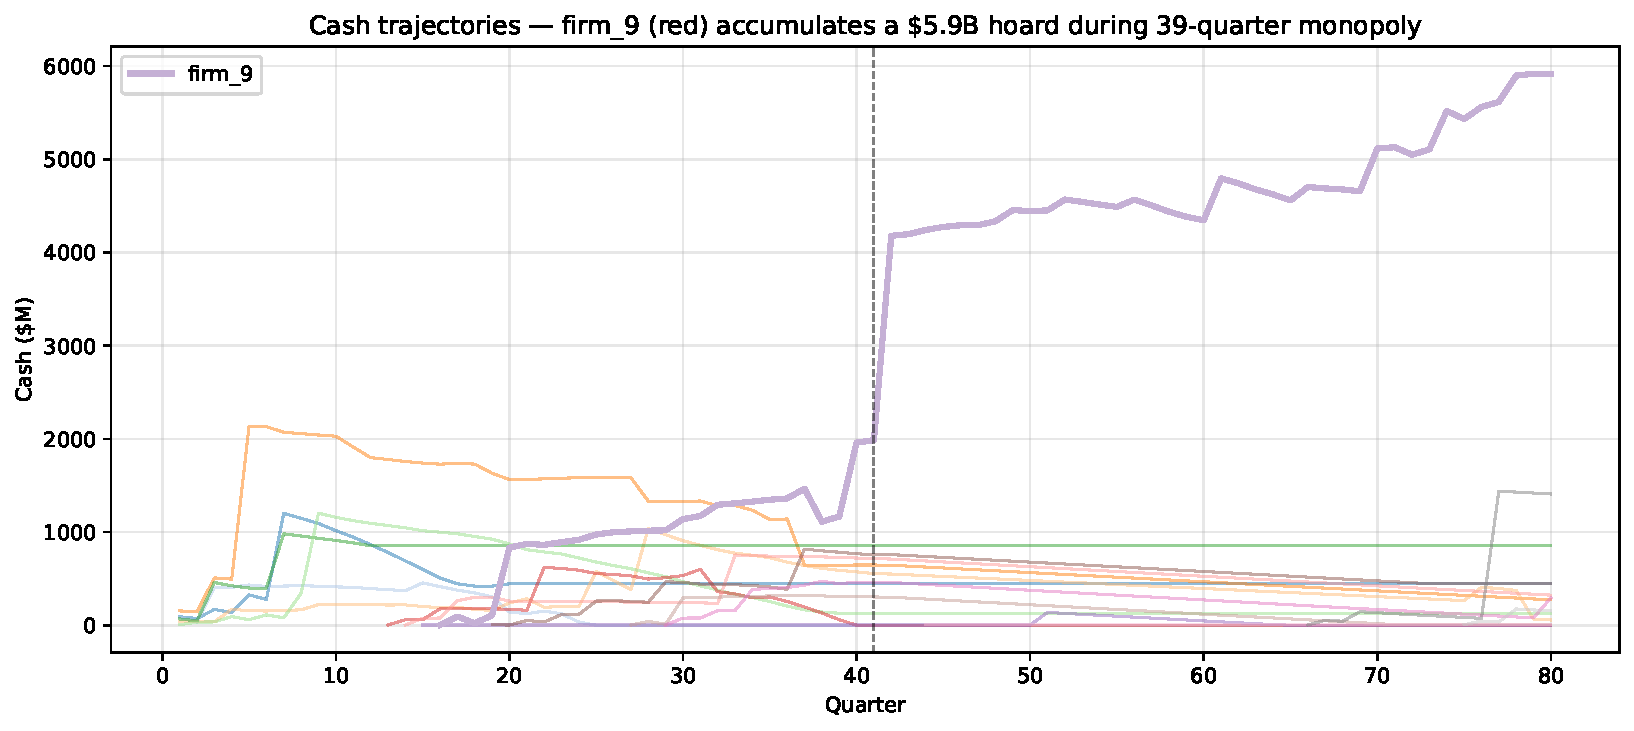
\includegraphics[width=\textwidth]{figures/cash}
\caption{Cash trajectories across all firms. firm\_9 (highlighted) accumulates a \$5.9B cash position through 39 quarters of monopoly profits. Several non-firm\_9 firms (firm\_2, firm\_5, firm\_14) maintain cash buffers above \$1B but do not deploy them to challenge the monopoly.}
\label{fig:cash}
\end{figure}

\paragraph{Behavioral IO and inattention.} \citet{Hortacsu2017} document that firms (and consumers) often exhibit inertia and inattention even when small adjustments would be profitable. \citet{Sims2003} provides the rational-inattention foundation. Our cash-flush incumbents' refusal to compete with firm\_9 has the feel of inattention --- they are not actively reasoning about a path back into competition --- but the LLMs do reason actively each quarter, so it is not a literal Sims-style inattention. It is closer to \citet{Gabaix2014}'s sparsity model, in which agents pay attention to a small set of dimensions: our firms appear to be focused on cash conservation rather than market reentry.

\section{The transition: equilibrium selection by an LLM}\label{sec:transition}

The most distinctive feature of the run is the transition between regimes. We argue that the equilibrium-selection mechanism is the environment LLM itself, acting as a focal-point selector \citep{Schelling1960,MailathPostlewaite1990} for the firm LLMs.

\paragraph{Schelling focal points.} \citet{Schelling1960} observed that in coordination games with multiple equilibria, players gravitate toward whichever equilibrium is most ``salient'' or ``focal,'' even when payoffs do not pin down a unique solution. Subsequent literature \citep{MailathPostlewaite1990,SugdenZamarron2006} has formalized this in evolutionary-game and learning settings. The standard story treats focality as a property of common knowledge or shared culture among players; in our setting, a different agent --- the environment LLM --- acts as the focal-point announcer. When the env interprets the post-Q41 firm decisions as ``the industry is consolidating around firm\_9'' and writes a narrative to that effect, that interpretation becomes common knowledge among the firm LLMs (who read the narrative the next quarter), and firms best-respond accordingly.

\paragraph{The procedural mechanism.} The environment LLM at each quarter receives firm decisions, the per-firm differentiation profiles, and a calibrator-anchored total demand. It returns per-firm shares and a narrative. From Q1 to Q40, the env's narratives describe a multi-firm market with regional segmentation. At Q41, when firm\_5 (Nordic + Benelux) defaults, the env's narrative shifts: it begins to describe firm\_9 as ``dominant.'' Once that narrative is in place, the env's subsequent allocations follow it: firm\_9 gets the demand, the other firms get zero. The differentiation attributes of the surviving firms (US Northeast, US Southeast, Western Europe, US Midwest) are still in the prompt context, but the env weighs them against the incumbent's narrative dominance and decides the niches no longer matter.

\paragraph{Why the simulation cannot escape.} An escape from the absorbing state would require either (i) firm\_9 itself losing market position (no mechanism: its cash buffer makes it default-immune), or (ii) the env's narrative interpretation flipping back to multi-firm competition (no mechanism: the env reads its own prior narratives as evidence). The simulation has entry, M\&A, and activist-investor mechanisms designed to exert pressure on monopolists, but they all route through the env LLM's interpretation of industry state, which has converged on ``firm\_9 owns this market.'' The leapfrog entries (Figure~\ref{fig:timeline}, bottom rows) document the failure: four sequential leapfrog candidates with elevated capability spawn, all stay dormant.

\paragraph{Connection to the LLM-agent literature.} Recent work on LLM-driven economic and social simulations has documented that LLM agents can exhibit emergent coordination on conventions and norms \citep{Park2023,AherArriagaKalai2023,Argyle2023}. \citet{Horton2023} explicitly proposes treating LLMs as ``simulated economic agents'' for behavioral economics. Our finding adds a wrinkle: in multi-LLM economies with a designated environment LLM, the env can act as a coordinating device that selects equilibria the firm-level LLMs would not necessarily select on their own. The selection mechanism is the env's narrative summary of past states, which becomes common knowledge by virtue of being included in every firm's prompt. This is, mechanically, very close to a Schelling focal point, but with an explicit agentic source rather than the cultural common-knowledge source of the canonical literature.

\paragraph{Why this matters for empirical IO.} Real-world equilibrium selection is hard to study because the focal point is rarely directly observable; one infers it from outcomes and structure. In our simulation, the focal-point selector is a single LLM whose narratives are logged. A researcher could read the env's actual prompts and outputs across the Q40--Q42 transition and document, sentence by sentence, when ``competitive'' phrasing gives way to ``consolidating'' phrasing. We have not done that here, but the data supports it.

\section{Anomalies and what does not fit}\label{sec:anomalies}

A precise reading requires noting where the simulation does \emph{not} resemble the empirical IO literature.

\paragraph{Speed of cascade.} Real coordination failures unfold over weeks to months. The 2007--2008 commercial-paper market freeze, often cited as the canonical modern coordination failure \citep{Brunnermeier2009}, took several weeks to fully manifest. Our cascade is one quarter wide. We attribute this to LLM tempo: each firm LLM evaluates the same Q41 default in parallel and best-responds in the same way, with no inertia or staggered adjustment.

\paragraph{Cash-rich firms refusing to compete.} Standard IO predicts that firms with positive variable margins and intact capacity continue producing as long as variable revenue covers variable cost, regardless of peer behavior. Our Q42--Q80 incumbents had cash, capacity, brand stocks, and differentiation profiles --- and chose zero output. The closest precedent is the literature on \emph{collusive standstill agreements} \citep{Tirole1988,FudenbergMaskin1986} where firms tacitly coordinate to restrict output. But tacit collusion would predict positive output at higher prices, not zero output. Our pattern is closer to a behavioral phenomenon for which we do not have a clean IO precedent.

\paragraph{No M\&A response.} The M\&A bidder LLM was active throughout the run. \citet{SalantSwitzerReynolds1983}'s merger paradox and the subsequent literature \citep{FarrellShapiro1990} predict that an industry with idle competitors is ripe for consolidating mergers --- the marginal value of an additional firm to the monopolist's portfolio is high, and the cash-rich monopolist could pick up competitors cheaply. We observed no M\&A activity in Phase 2; the bidder LLM, reading the same monopoly narrative as the env, judged that firm\_9 had no incentive to acquire what was not threatening it.

\paragraph{No leapfrog success.} The empirical leapfrog literature \citep{FudenbergGilbertStiglitzTirole1983,VivesInnovation2008} documents real cases of incumbents being displaced by technologically distinct entrants. Our four leapfrog candidates failed not because their technology was inadequate but because PE refused to fund them. This is a finance-side failure, not a technology-side failure, and the simulation lacks any mechanism by which a sufficiently determined founder could bypass the PE bottleneck (e.g., bootstrapping, debt, alternative funding).

\paragraph{No Schumpeterian creative destruction.} \citet{Schumpeter1942} and the modern creative-destruction literature \citep{AghionHowitt1992,AghionEtAl2005} emphasize that monopoly is typically temporary --- the very profits that flow to the monopolist attract challengers and incentivize incumbents to invest in maintaining their position. Our firm\_9 invested neither in defending its position (no R\&D acceleration after Q42) nor in advancing the technology frontier (no Gen-2 push). The simulation's monopoly is purely rentier: extraction without investment. This may reflect the absence of an exogenous threat the LLMs could perceive.

\paragraph{No regulatory response.} The SEC LLM was active throughout. Real-world antitrust enforcement \citep{Whinston2007,KhanAmazon2017} would view a 39-quarter monopoly with HHI = 10{,}000 as worth investigating. Our SEC LLM never opened a Phase-2 investigation into firm\_9; it was prompted to look for accounting and disclosure anomalies, not for monopolization, and the antitrust dimension is not in its prompt.

\section{Implications for LLM-generated economic data as research artifact}\label{sec:research_use}

The simulation is one run, with one seed, and one set of LLM models. We are cautious about generalizing. But the run does suggest several uses for LLM-generated IO data.

\paragraph{Equilibrium-selection studies.} The Q40--Q42 transition is, to our knowledge, an unusually clean instance of an industry flipping between equilibria with all firm primitives observable and unchanged. Empirically, such transitions are very hard to study: real industries typically have unobserved heterogeneity that contaminates ``before'' and ``after'' comparisons. Researchers working on coordination-failure mechanisms (\citealp{CooperJohn1988,Cooper1999}; \citealp{ChamleyGale1994} for sequential investment cascades) could use this run as a clean test case for cascade-prediction models.

\paragraph{Text-as-data on board minutes and annual reports.} The simulation produces self-justified board minutes, annual reports, and analyst notes for every firm at every quarter. The text contains explicit reasoning about competitive position, capital allocation, and strategic choice. This is comparable in form to the corporate-disclosure text used by \citet{LoughranMcDonald2011} in finance text-as-data work, but with the advantage that the underlying primitives are observable. A researcher could test, for instance, whether soft text indicators (sentiment, hedging, optimism) predict subsequent firm-level outcomes when the latent state is known.

\paragraph{Entry-deterrence under perceived monopoly.} Phase 2 of the simulation is essentially a controlled experiment in entry deterrence by perception. The four sequential leapfrog spawns held capability advantages over the incumbent --- and none was funded. Researchers studying VC dry-powder cycles \citep{KortumLerner2000,GompersLerner2001} could use the run's PE-decision logs to study how AI investors interpret ambiguous signals about market openness.

\paragraph{Caveats.} (i) One run, one seed: the Q41 cascade may be path-dependent on the specific firm that defaulted and the env LLM's reasoning priors. (ii) LLM tempo compresses real-world dynamics. (iii) The simulation has no exogenous macro shocks, which in real industries periodically dislodge absorbing states. (iv) The prompts encode design choices (e.g., the env's instruction to respect heterogeneous consumer preferences) that bias the regime; a different prompt would generate different equilibria. None of these caveats undercut the run's value as an artifact, but they do constrain claims of generality.

\section{Synthesis: phenomena and theory}

Table~\ref{tab:synthesis} summarizes the mapping from observed simulation phenomena to literature, with a column indicating fit quality.

\begin{table}[h]
\centering
\small
\begin{tabular}{p{4.2cm}p{5.5cm}p{1.4cm}p{3.0cm}}
\toprule
\textbf{Observed phenomenon} & \textbf{Theoretical/empirical reference} & \textbf{Fit} & \textbf{Comment} \\
\midrule
Multi-firm differentiated equilibrium with regional niches (Q1--Q40) & \citet{Hotelling1929,Salop1979,dAspremontGabszewiczThisse1979} & strong & The simulation literally implements geographic differentiation \\
Equilibrium share dispersion (top firm 16--26\%) & \citet{BerryLevinsohnPakes1995,Nevo2001} & strong & Env LLM acts as procedural BLP \\
Equilibrium count of 8--9 firms in mature regime & \citet{BresnahanReiss1991,Sutton1991} & strong & Entry judge converges to count \\
Entry / exit / replacement churn & \citet{Klepper1996,Hopenhayn1992,Jovanovic1982} & partial & Tempo compressed; selection less productivity-driven \\
Q41 single default $\to$ Q42 industry-wide retreat & \citet{CooperJohn1988,DiamondDybvig1983} & strong & Textbook coordination failure \\
Cash-flush firms refusing to compete & \citet{Tirole1988,FudenbergMaskin1986} (tacit collusion) & weak & Output is zero, not restricted; no clean precedent \\
Persistent monopoly under perceived dominance & \citet{Sutton1991} (endogenous sunk costs) & moderate & Mechanism is finance-side, not strategic \\
Leapfrog entrants fail to attract funding & \citet{Gompers1995,GompersLerner2001,KortumLerner2000} & strong & Dry-powder withdrawal exactly as Gompers et al.\ describe \\
Cash hoarding by monopolist with no strategic deployment & \citet{BatesKahleStulz2009} & moderate & Precautionary motive unclear; no obvious risk \\
No M\&A consolidation in absorbing state & \citet{SalantSwitzerReynolds1983,FarrellShapiro1990} & contradicts & Theory predicts mergers; we observe none \\
No Schumpeterian creative destruction & \citet{Schumpeter1942,AghionHowitt1992} & contradicts & No incumbent investment; no challenger displaces \\
No regulatory antitrust response & \citet{Whinston2007,KhanAmazon2017} & N/A & SEC LLM not prompted on antitrust \\
LLM env acts as equilibrium-selection focal point & \citet{Schelling1960,MailathPostlewaite1990} & novel & Standard theory has no agentic focal-point selector \\
\bottomrule
\end{tabular}
\caption{Mapping from observed phenomena in the Wave $\nu+6$ simulation to canonical references. ``Fit'' is the author's qualitative judgment of how cleanly the simulation reproduces what the reference predicts, ranging from \emph{strong} (textbook implementation) through \emph{moderate} and \emph{partial} to \emph{contradicts}. The bottom row marks the most novel finding.}
\label{tab:synthesis}
\end{table}

\section{Closing}

The Wave $\nu+6$ run produces, in 80 simulated quarters, a clean exhibition of horizontal-differentiation equilibrium followed by a clean exhibition of coordination-failure collapse, connected by an equilibrium-selection event whose mechanism is an LLM agent's narrative interpretation. Each phase maps onto an established branch of the IO literature with high fidelity; the transition is novel and points to LLM-as-focal-point as a coordination mechanism worth further study. As empirical material, the run's value is not in confirming what the literature already knows --- though it does that --- but in exhibiting transitions and mechanisms that real data only ever shows partially.

\bibliographystyle{plainnat}

\begin{thebibliography}{99}

\bibitem[Acemoglu et~al.(2015)]{Acemoglu2015}
Acemoglu, D., Ozdaglar, A., \& Tahbaz-Salehi, A. (2015).
\newblock Systemic risk and stability in financial networks.
\newblock \emph{American Economic Review}, 105(2), 564--608.

\bibitem[Aghion \& Howitt(1992)]{AghionHowitt1992}
Aghion, P., \& Howitt, P. (1992).
\newblock A model of growth through creative destruction.
\newblock \emph{Econometrica}, 60(2), 323--351.

\bibitem[Aghion et~al.(2005)]{AghionEtAl2005}
Aghion, P., Bloom, N., Blundell, R., Griffith, R., \& Howitt, P. (2005).
\newblock Competition and innovation: An inverted-U relationship.
\newblock \emph{Quarterly Journal of Economics}, 120(2), 701--728.

\bibitem[Aher et~al.(2023)]{AherArriagaKalai2023}
Aher, G., Arriaga, R.~I., \& Kalai, A.~T. (2023).
\newblock Using large language models to simulate multiple humans and replicate human subject studies.
\newblock In \emph{International Conference on Machine Learning}.

\bibitem[Allen \& Gale(2000)]{AllenGale2000}
Allen, F., \& Gale, D. (2000).
\newblock Financial contagion.
\newblock \emph{Journal of Political Economy}, 108(1), 1--33.

\bibitem[Argyle et~al.(2023)]{Argyle2023}
Argyle, L.~P., Busby, E.~C., Fulda, N., Gubler, J., Rytting, C., \& Wingate, D. (2023).
\newblock Out of one, many: Using language models to simulate human samples.
\newblock \emph{Political Analysis}, 31(3), 337--351.

\bibitem[Bain(1956)]{Bain1956}
Bain, J.~S. (1956).
\newblock \emph{Barriers to New Competition}.
\newblock Harvard University Press.

\bibitem[Barney(1991)]{Barney1991}
Barney, J. (1991).
\newblock Firm resources and sustained competitive advantage.
\newblock \emph{Journal of Management}, 17(1), 99--120.

\bibitem[Bates et~al.(2009)]{BatesKahleStulz2009}
Bates, T.~W., Kahle, K.~M., \& Stulz, R.~M. (2009).
\newblock Why do U.S.\ firms hold so much more cash than they used to?
\newblock \emph{Journal of Finance}, 64(5), 1985--2021.

\bibitem[Berry(1994)]{Berry1994}
Berry, S.~T. (1994).
\newblock Estimating discrete-choice models of product differentiation.
\newblock \emph{RAND Journal of Economics}, 25(2), 242--262.

\bibitem[Berry et~al.(1995)]{BerryLevinsohnPakes1995}
Berry, S., Levinsohn, J., \& Pakes, A. (1995).
\newblock Automobile prices in market equilibrium.
\newblock \emph{Econometrica}, 63(4), 841--890.

\bibitem[Berry \& Haile(2014)]{BerryHaileSurvey2014}
Berry, S., \& Haile, P. (2014).
\newblock Identification in differentiated products markets using market level data.
\newblock \emph{Econometrica}, 82(5), 1749--1797.

\bibitem[Bloom(2009)]{Bloom2009}
Bloom, N. (2009).
\newblock The impact of uncertainty shocks.
\newblock \emph{Econometrica}, 77(3), 623--685.

\bibitem[Bloom et~al.(2018)]{BloomFloetottoJaimovichSaportaEksten2018}
Bloom, N., Floetotto, M., Jaimovich, N., Saporta-Eksten, I., \& Terry, S.~J. (2018).
\newblock Really uncertain business cycles.
\newblock \emph{Econometrica}, 86(3), 1031--1065.

\bibitem[Bresnahan \& Reiss(1991)]{BresnahanReiss1991}
Bresnahan, T.~F., \& Reiss, P.~C. (1991).
\newblock Entry and competition in concentrated markets.
\newblock \emph{Journal of Political Economy}, 99(5), 977--1009.

\bibitem[Brunnermeier(2009)]{Brunnermeier2009}
Brunnermeier, M.~K. (2009).
\newblock Deciphering the liquidity and credit crunch 2007--2008.
\newblock \emph{Journal of Economic Perspectives}, 23(1), 77--100.

\bibitem[Chamley \& Gale(1994)]{ChamleyGale1994}
Chamley, C., \& Gale, D. (1994).
\newblock Information revelation and strategic delay in a model of investment.
\newblock \emph{Econometrica}, 62(5), 1065--1085.

\bibitem[Cooper(1999)]{Cooper1999}
Cooper, R.~W. (1999).
\newblock \emph{Coordination Games: Complementarities and Macroeconomics}.
\newblock Cambridge University Press.

\bibitem[Cooper \& John(1988)]{CooperJohn1988}
Cooper, R., \& John, A. (1988).
\newblock Coordinating coordination failures in Keynesian models.
\newblock \emph{Quarterly Journal of Economics}, 103(3), 441--463.

\bibitem[d'Aspremont et~al.(1979)]{dAspremontGabszewiczThisse1979}
d'Aspremont, C., Gabszewicz, J.~J., \& Thisse, J.-F. (1979).
\newblock On Hotelling's `stability in competition'.
\newblock \emph{Econometrica}, 47(5), 1145--1150.

\bibitem[Diamond \& Dybvig(1983)]{DiamondDybvig1983}
Diamond, D.~W., \& Dybvig, P.~H. (1983).
\newblock Bank runs, deposit insurance, and liquidity.
\newblock \emph{Journal of Political Economy}, 91(3), 401--419.

\bibitem[Dixit(1980)]{Dixit1980}
Dixit, A. (1980).
\newblock The role of investment in entry-deterrence.
\newblock \emph{Economic Journal}, 90(357), 95--106.

\bibitem[Dixit \& Pindyck(1994)]{DixitPindyck1994}
Dixit, A.~K., \& Pindyck, R.~S. (1994).
\newblock \emph{Investment under Uncertainty}.
\newblock Princeton University Press.

\bibitem[Ericson \& Pakes(1995)]{EricsonPakes1995}
Ericson, R., \& Pakes, A. (1995).
\newblock Markov-perfect industry dynamics: A framework for empirical work.
\newblock \emph{Review of Economic Studies}, 62(1), 53--82.

\bibitem[Farrell \& Shapiro(1990)]{FarrellShapiro1990}
Farrell, J., \& Shapiro, C. (1990).
\newblock Horizontal mergers: An equilibrium analysis.
\newblock \emph{American Economic Review}, 80(1), 107--126.

\bibitem[Fudenberg et~al.(1983)]{FudenbergGilbertStiglitzTirole1983}
Fudenberg, D., Gilbert, R., Stiglitz, J., \& Tirole, J. (1983).
\newblock Preemption, leapfrogging and competition in patent races.
\newblock \emph{European Economic Review}, 22(1), 3--31.

\bibitem[Fudenberg \& Maskin(1986)]{FudenbergMaskin1986}
Fudenberg, D., \& Maskin, E. (1986).
\newblock The folk theorem in repeated games with discounting or with incomplete information.
\newblock \emph{Econometrica}, 54(3), 533--554.

\bibitem[Gabaix(2014)]{Gabaix2014}
Gabaix, X. (2014).
\newblock A sparsity-based model of bounded rationality.
\newblock \emph{Quarterly Journal of Economics}, 129(4), 1661--1710.

\bibitem[Ghemawat(1991)]{Ghemawat1991}
Ghemawat, P. (1991).
\newblock \emph{Commitment: The Dynamic of Strategy}.
\newblock Free Press.

\bibitem[Gompers(1995)]{Gompers1995}
Gompers, P.~A. (1995).
\newblock Optimal investment, monitoring, and the staging of venture capital.
\newblock \emph{Journal of Finance}, 50(5), 1461--1489.

\bibitem[Gompers \& Lerner(2001)]{GompersLerner2001}
Gompers, P., \& Lerner, J. (2001).
\newblock The venture capital revolution.
\newblock \emph{Journal of Economic Perspectives}, 15(2), 145--168.

\bibitem[Hopenhayn(1992)]{Hopenhayn1992}
Hopenhayn, H.~A. (1992).
\newblock Entry, exit, and firm dynamics in long run equilibrium.
\newblock \emph{Econometrica}, 60(5), 1127--1150.

\bibitem[Horta\c{c}su et~al.(2017)]{Hortacsu2017}
Horta\c{c}su, A., Madanizadeh, S.~A., \& Puller, S.~L. (2017).
\newblock Power to choose? An analysis of consumer inertia in the residential electricity market.
\newblock \emph{American Economic Journal: Economic Policy}, 9(4), 192--226.

\bibitem[Horton(2023)]{Horton2023}
Horton, J.~J. (2023).
\newblock Large language models as simulated economic agents: What can we learn from \emph{homo silicus}?
\newblock NBER Working Paper 31122.

\bibitem[Hotelling(1929)]{Hotelling1929}
Hotelling, H. (1929).
\newblock Stability in competition.
\newblock \emph{Economic Journal}, 39(153), 41--57.

\bibitem[Jovanovic(1982)]{Jovanovic1982}
Jovanovic, B. (1982).
\newblock Selection and the evolution of industry.
\newblock \emph{Econometrica}, 50(3), 649--670.

\bibitem[Kaplan \& Str\"omberg(2003)]{KaplanStromberg2003}
Kaplan, S.~N., \& Str\"omberg, P. (2003).
\newblock Financial contracting theory meets the real world: An empirical analysis of venture capital contracts.
\newblock \emph{Review of Economic Studies}, 70(2), 281--315.

\bibitem[Khan(2017)]{KhanAmazon2017}
Khan, L.~M. (2017).
\newblock Amazon's antitrust paradox.
\newblock \emph{Yale Law Journal}, 126(3), 710--805.

\bibitem[Klepper(1996)]{Klepper1996}
Klepper, S. (1996).
\newblock Entry, exit, growth, and innovation over the product life cycle.
\newblock \emph{American Economic Review}, 86(3), 562--583.

\bibitem[Klepper \& Graddy(1990)]{KlepperGraddy1990}
Klepper, S., \& Graddy, E. (1990).
\newblock The evolution of new industries and the determinants of market structure.
\newblock \emph{RAND Journal of Economics}, 21(1), 27--44.

\bibitem[Kortum \& Lerner(2000)]{KortumLerner2000}
Kortum, S., \& Lerner, J. (2000).
\newblock Assessing the contribution of venture capital to innovation.
\newblock \emph{RAND Journal of Economics}, 31(4), 674--692.

\bibitem[Loughran \& McDonald(2011)]{LoughranMcDonald2011}
Loughran, T., \& McDonald, B. (2011).
\newblock When is a liability not a liability? Textual analysis, dictionaries, and 10-Ks.
\newblock \emph{Journal of Finance}, 66(1), 35--65.

\bibitem[Mailath \& Postlewaite(1990)]{MailathPostlewaite1990}
Mailath, G.~J., \& Postlewaite, A. (1990).
\newblock Asymmetric information bargaining problems with many agents.
\newblock \emph{Review of Economic Studies}, 57(3), 351--367.

\bibitem[Nevo(2001)]{Nevo2001}
Nevo, A. (2001).
\newblock Measuring market power in the ready-to-eat cereal industry.
\newblock \emph{Econometrica}, 69(2), 307--342.

\bibitem[Park et~al.(2023)]{Park2023}
Park, J.~S., O'Brien, J., Cai, C.~J., Morris, M.~R., Liang, P., \& Bernstein, M.~S. (2023).
\newblock Generative agents: Interactive simulacra of human behavior.
\newblock In \emph{Proceedings of UIST 2023}.

\bibitem[Porter(1980)]{Porter1980}
Porter, M.~E. (1980).
\newblock \emph{Competitive Strategy: Techniques for Analyzing Industries and Competitors}.
\newblock Free Press.

\bibitem[Salant et~al.(1983)]{SalantSwitzerReynolds1983}
Salant, S.~W., Switzer, S., \& Reynolds, R.~J. (1983).
\newblock Losses from horizontal merger.
\newblock \emph{Quarterly Journal of Economics}, 98(2), 185--199.

\bibitem[Salop(1979)]{Salop1979}
Salop, S.~C. (1979).
\newblock Monopolistic competition with outside goods.
\newblock \emph{Bell Journal of Economics}, 10(1), 141--156.

\bibitem[Schelling(1960)]{Schelling1960}
Schelling, T.~C. (1960).
\newblock \emph{The Strategy of Conflict}.
\newblock Harvard University Press.

\bibitem[Schumpeter(1942)]{Schumpeter1942}
Schumpeter, J.~A. (1942).
\newblock \emph{Capitalism, Socialism and Democracy}.
\newblock Harper.

\bibitem[Sims(2003)]{Sims2003}
Sims, C.~A. (2003).
\newblock Implications of rational inattention.
\newblock \emph{Journal of Monetary Economics}, 50(3), 665--690.

\bibitem[Spence(1977)]{Spence1977}
Spence, A.~M. (1977).
\newblock Entry, capacity, investment and oligopolistic pricing.
\newblock \emph{Bell Journal of Economics}, 8(2), 534--544.

\bibitem[Sugden \& Zamarr\'on(2006)]{SugdenZamarron2006}
Sugden, R., \& Zamarr\'on, I.~E. (2006).
\newblock Finding the key: The riddle of focal points.
\newblock \emph{Journal of Economic Psychology}, 27(5), 609--621.

\bibitem[Sutton(1991)]{Sutton1991}
Sutton, J. (1991).
\newblock \emph{Sunk Costs and Market Structure}.
\newblock MIT Press.

\bibitem[Tirole(1988)]{Tirole1988}
Tirole, J. (1988).
\newblock \emph{The Theory of Industrial Organization}.
\newblock MIT Press.

\bibitem[Vives(2008)]{VivesInnovation2008}
Vives, X. (2008).
\newblock Innovation and competitive pressure.
\newblock \emph{Journal of Industrial Economics}, 56(3), 419--469.

\bibitem[Wernerfelt(1984)]{Wernerfelt1984}
Wernerfelt, B. (1984).
\newblock A resource-based view of the firm.
\newblock \emph{Strategic Management Journal}, 5(2), 171--180.

\bibitem[Whinston(2007)]{Whinston2007}
Whinston, M.~D. (2007).
\newblock Antitrust policy toward horizontal mergers.
\newblock In \emph{Handbook of Industrial Organization}, vol.~3, 2369--2440.

\end{thebibliography}

\end{document}
